\section{System Demonstration}

% The system as shown as \figref{fig:demo_ov} comprises five primary pages: The Instruction Page offers an overview of the system's functionality and usage instructions; Phoneme Page displays a 2D distribution graph of the 50 canine phoneme cluster nodes. 
% derived from self-supervised learning and clustering, alongside corresponding audio examples; Vocabulary Page showcases the vocabulary list filtered through plausible score, presenting words with associated video and audio examples; Test Your Data Page enables users to upload videos or audio files for transcription results, allowing them to listen to phoneme sounds by clicking on the waveform.
The system as shown as \figref{fig:demo_ov} comprises four primary modules: phoneme module, vocabulary module, test your data module, and example module.
Phoneme module displays a 2D distribution graph of the 50 canine phoneme cluster nodes derived from self-supervised learning and clustering, alongside corresponding audio examples; 
Vocabulary module showcases the vocabulary list filtered through plausible score, presenting words with associated video and audio examples; 
Test your data module enables users to upload videos or audio files for transcription results, allowing them to listen to phoneme sounds by clicking on the waveform;
Example module displays the transcription results of 10 randomly selected dog vocalization clips.
% \MY{we can focus on introducing different functions this system has, instead of introducing them as ``pages''. you can give a full pipeline figure first on what this system can do (put different modules in block and use arrows to link them), or a list of functions, then introduce each part, since our system does follow an order. }
\begin{figure}[th]
    \centering
    \scalebox{0.30}{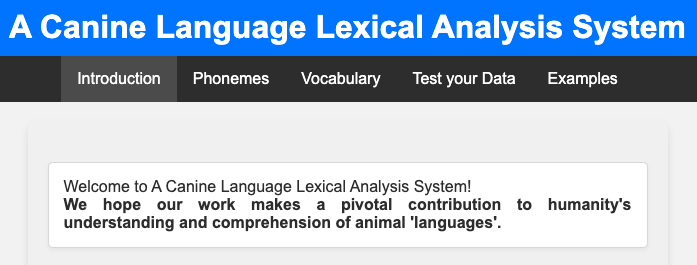
\includegraphics{demo_overview.png}}
    \caption{Instruction Page in Demo}
    \label{fig:demo_ov}
\end{figure}

\begin{figure}[th]
    \centering
    \scalebox{0.35}{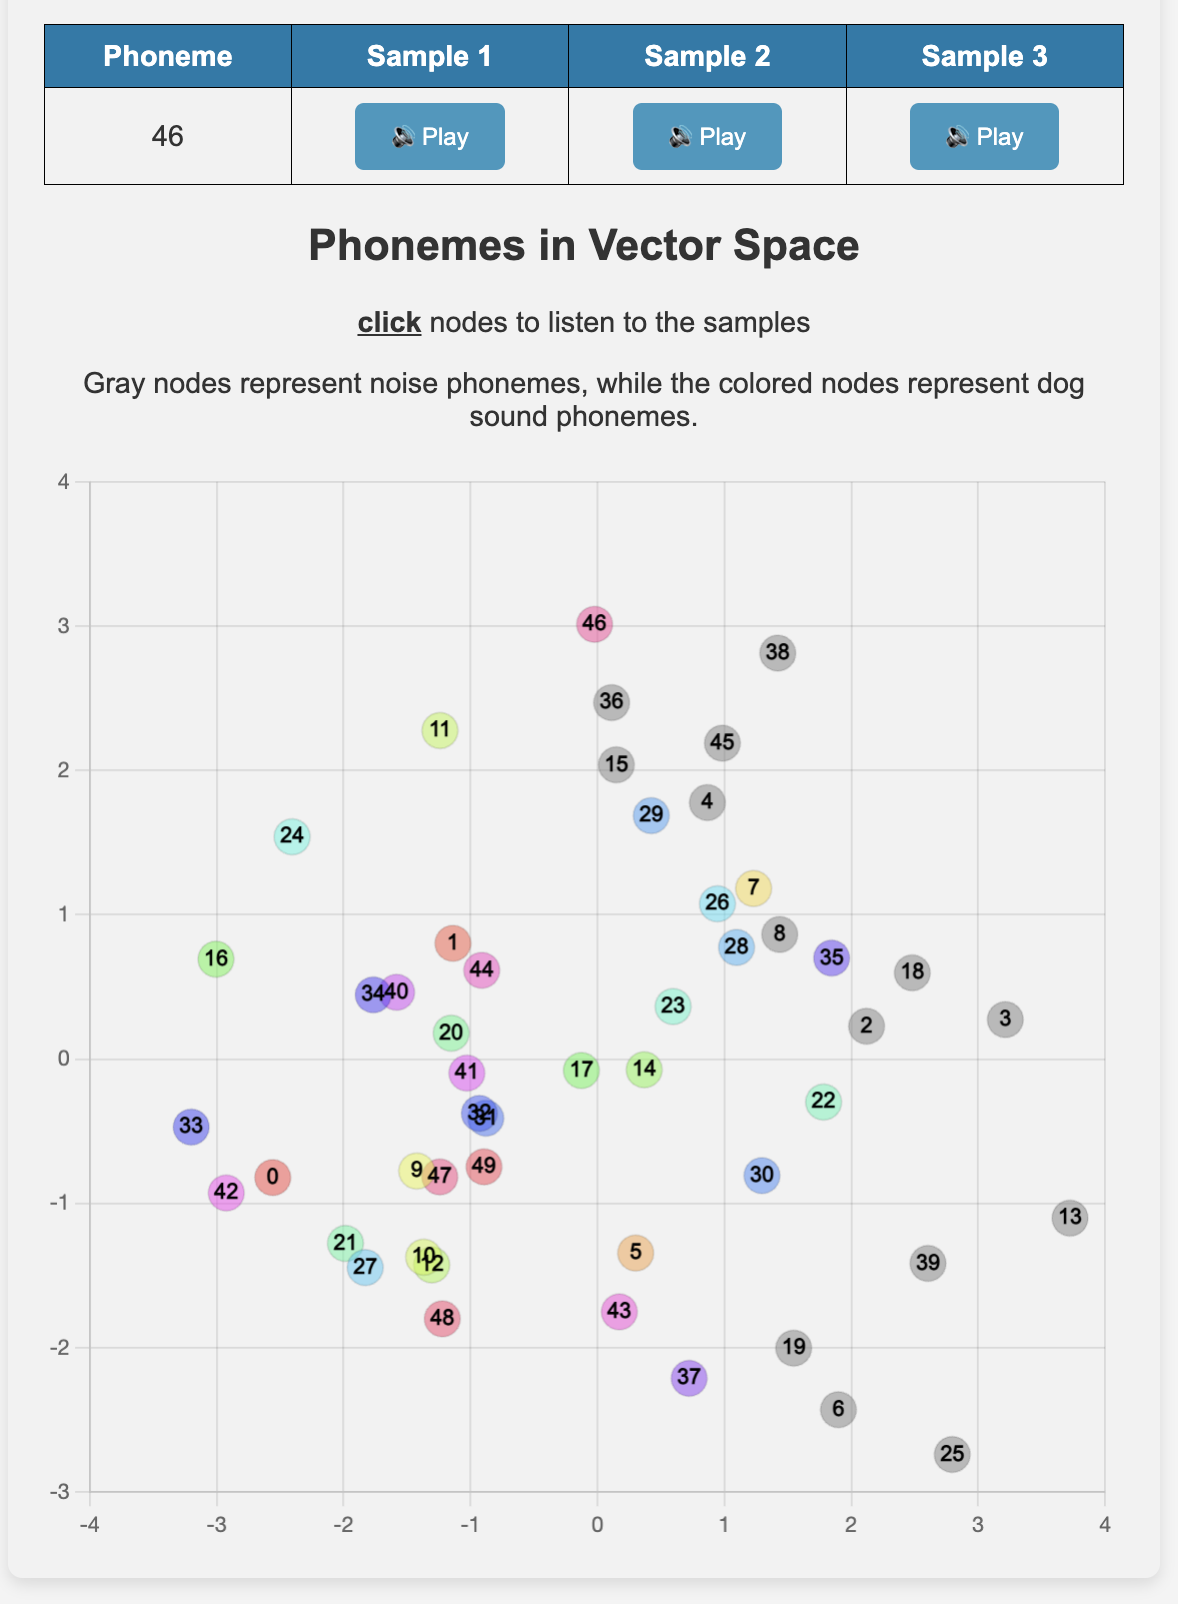
\includegraphics{demo-phonemes.png}}
    \caption{Phoneme Module Demonstration}\label{fig:demo_p}
\end{figure}

\begin{figure}[th]
    \centering
    \scalebox{0.22}{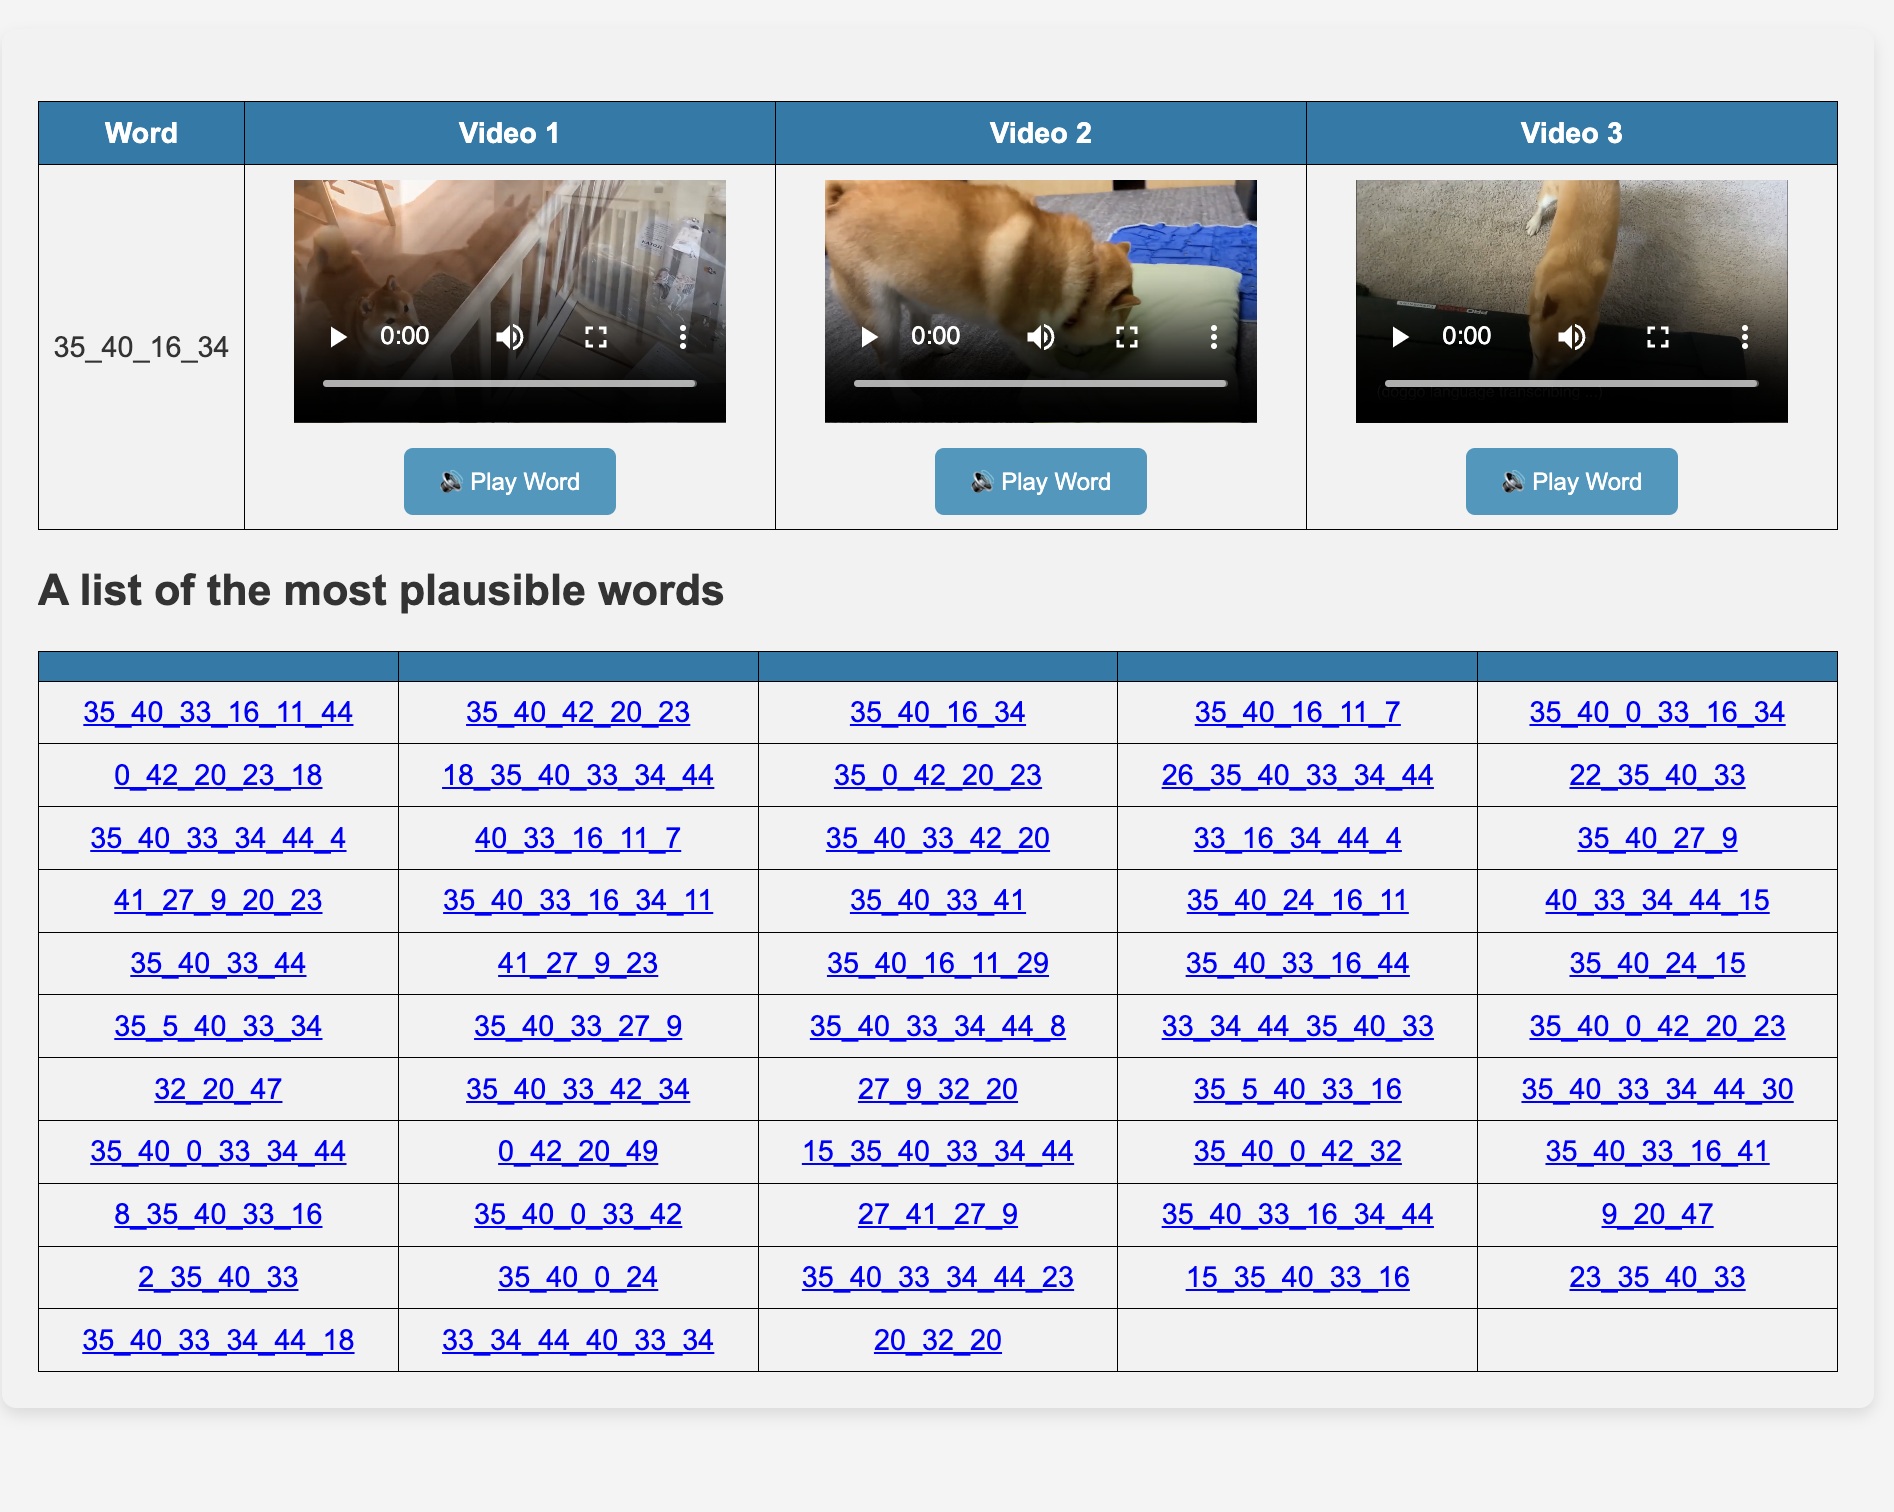
\includegraphics{demo_vocabulary.png}}
    \caption{Vocabulary Module Demonstration}
    \label{fig:demo_v}
\end{figure}

\begin{figure}[th]
    \centering
    \scalebox{0.4}{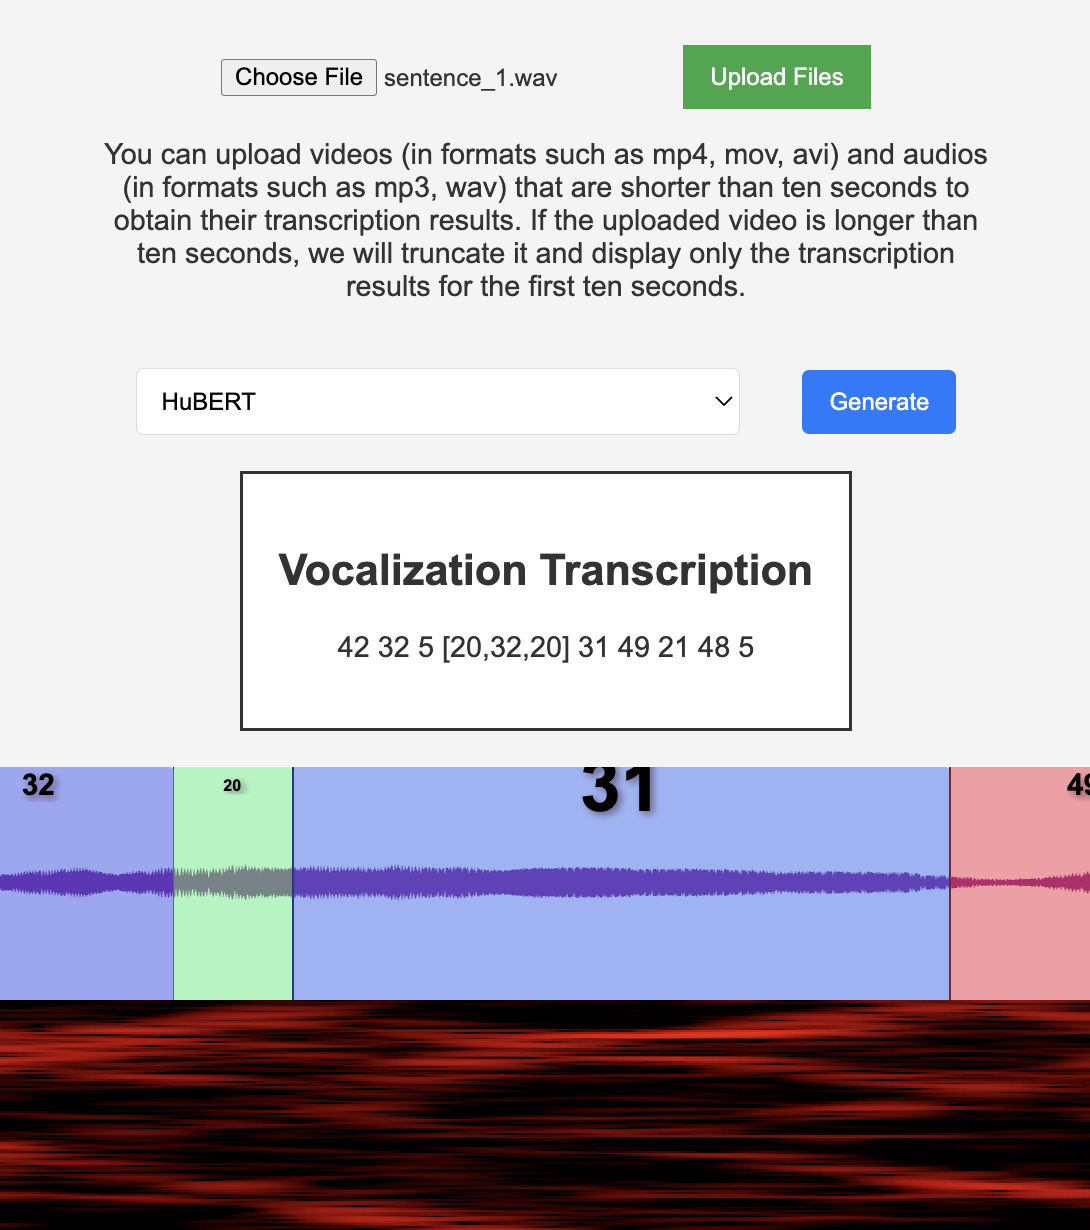
\includegraphics{demo_test2.png}}
    \caption{Test your data Module Demonstration}
    \label{fig:demo_t1}
\end{figure}

\subsection{Phoneme Module}

As \figref{fig:demo_p} shown, the Phoneme module aims to illustrate the spatial distribution and relative positioning of the 50 distinct phoneme nodes. Users can click on each cluster node to listen to examples. Color-coded centroids represent canine phonemes, while gray nodes represent noise phonemes. Despite noise reduction techniques, complete elimination of noise remains unattainable. Users can identify similar phonemes by listening to audio examples of adjacent cluster nodes.

\subsection{Vocabulary Module}

As \figref{fig:demo_v} shown, the Vocabulary module functions similarly to the Phoneme module, providing the most probable canine lexical vocabulary sorted by plausible score and represented by cluster centroid numbers. To better explore the context of each word, we offer not only example audio but also accompanying videos extended by 0.5 seconds before and after for user observation.

\subsection{Test Your Data Module}

As \figref{fig:demo_t1} shown, in this module, users can upload videos or audio files and choose the transcription method to obtain the transcription results of the canine audio within. However, it's important to note that to ensure smooth server operation, videos or audio longer than 10 seconds will be truncated, retaining only the first 10 seconds for transcription. The page will display the translation results alongside the corresponding audio waveform, allowing users to click on segments corresponding to phonemes to listen to the audio.

\subsection{Example Module}

In this module, we have prepared 10 randomly selected dog vocalization clips for users who do not currently have dog audio. Users can select a sound clip from the dropdown menu, listen to it, and observe the transcription results generated by two different methods.
